\section{观测与拟合目标}
\label{sec:opt-fit-observations}

章首的两条曲线说明，拟合问题至少由三样东西决定：允许选哪些函数，读到了函数的什么信息，以及读数与候选不完全相合时怎样计价。本节先把候选与观测写成数学对象，分清“数据能确定什么”与“我们额外偏好什么”；再比较几种残差代价与正则化；最后检查一个容易混淆的实例：把二次惩罚加进目标与在更新规则中直接收缩参数，是不是同一件事。

\subsection{有限观测与候选函数}
\label{sec:opt-fit-finite-observations}

\paragraph{候选集合与观测映射}
设我们在$x=0,\tfrac12,1$三处读到某个函数的值$0,1,0$。要从中“恢复”函数，先得说清从哪里找：可以是次数不超过$3$的多项式，也可以是$[0,1]$上所有连续函数，或某个函数空间。把允许的函数组成的集合称为候选集合，记作$C$。读数由一条规则从函数算出，这里是$f\mapsto(f(0),f(\tfrac12),f(1))$。一般地，称$L:C\to\mathbb R^n$，$Lf=(L_1f,\dots,L_nf)^\top$为\term{观测映射}（observation map），$\bm y\in\mathbb R^n$为数据，拟合就是在$C$中找$f$使$Lf$与$\bm y$相合或相近。

读数不必是点值。区间平均$L_if=(b-a)^{-1}\int_a^bf\,\mathrm dx$、加权积分$\int_0^1f\varphi_i\,\mathrm dx$都是关于$f$线性的读数，本章主要讨论这样的\emph{线性观测}：每个$L_i$对线性组合保持线性，$L_i(\alpha f+\beta g)=\alpha L_if+\beta L_ig$。

\paragraph{观测与候选空间必须相容}
同一条读取规则放在不同的候选空间里，可能根本没有意义。$L^2(0,1)$的元素是几乎处处相等的函数组成的等价类，改动一个点的值不改变元素本身，所以“在$x=\tfrac12$处取值”在$L^2(0,1)$上没有良定义。积分读数则不同：由Cauchy--Schwarz不等式，$\bigl|\int_a^bf\,\mathrm dx\bigr|\le\sqrt{b-a}\,\|f\|_{L^2}$，它在$L^2$上有定义且连续。若把候选放进再生核Hilbert空间$H_K$，点值读数满足$|f(x)|\le\sqrt{K(x,x)}\,\|f\|_{H_K}$，是有界线性泛函；这一性质以及核截面、Gram矩阵与核积分算子的谱展开，可参考\BookChapterRef{chap:rkhs}{卷二“再生核Hilbert空间”章}，本章第~\ref{sec:opt-fit-hilbert}节和第~\ref{sec:opt-fit-global}节会反复用到。所以写下拟合问题之前，先要核对每个$L_i$在$C$上是否有定义，必要时是否连续。

\paragraph{有解、唯一与可识别}
给定观测映射以后，有三个不同的问题。第一，方程$Lf=\bm y$在$C$中是否有解，即$\bm y$是否属于像集$L(C)$。第二，对这一组具体数据，解是否唯一。第三，不论数据取什么值，$L$在$C$上是否单射，即读数是否总能区分两个不同的候选。前两个问题依赖于$\bm y$，第三个只依赖于$C$与$L$。

\begin{lemma}[读数区分全部候选的条件]
\label{lem:opt-fit-identifiability}
设$C$是线性空间$V$的子集，$L:V\to\mathbb R^n$线性。记$C-C=\{f-g:f,g\in C\}$。则$L$在$C$上单射，当且仅当$(C-C)\cap\ker L=\{0\}$。
\end{lemma}

\begin{proof}
对$f,g\in C$，由线性，$Lf=Lg$当且仅当$f-g\in\ker L$。若$(C-C)\cap\ker L=\{0\}$，则$Lf=Lg$推出$f-g=0$。反之，若有非零的$f-g\in(C-C)\cap\ker L$，则$f\ne g$而$Lf=Lg$，单射不成立。
\end{proof}

当$C$本身是线性子空间时，$C-C=C$，条件化为$C\cap\ker L=\{0\}$。取$C$为次数不超过$3$的多项式，三个点值读数不能区分全部候选：$p(x)=x(x-\tfrac12)(x-1)$非零，却在三个观测点处都等于零。于是$f_0(x)=4x(1-x)$与$f_0+c\,p$对每个实数$c$都给出同样的读数$(0,1,0)$。图~\ref{fig:opt-fit-invisible-direction}画出了$c=0,\pm8,\pm16$的五条曲线：它们在三个黑点处重合，在点与点之间沿$p$的方向任意偏移。$p$所在的方向对这组读数完全不可见。

\begin{figure}[!htbp]
  \centering
  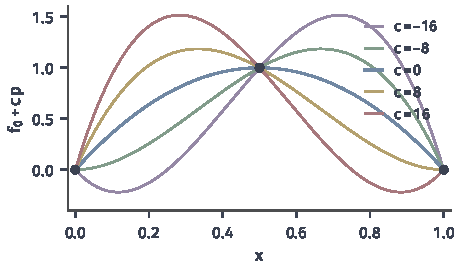
\includegraphics[width=78mm]{figures/03-optimization-evolution-and-signals/01-optimization/matplotlib/c8-invisible-direction/figure.pdf}
  \caption{观测不可见的方向。在次数不超过$3$的多项式中，$f_0(x)=4x(1-x)$与$f_0+c\,p$（$p(x)=x(x-\tfrac12)(x-1)$，$c=0,\pm8,\pm16$）在$x=0,\tfrac12,1$处的读数都是$0,1,0$（黑点）。$p$属于观测映射的零空间，读数无法区分这些候选。}
  \label{fig:opt-fit-invisible-direction}
\end{figure}

\paragraph{惩罚只提供选解偏好}
在这条直线$\{f_0+c\,p:c\in\mathbb R\}$上，若偏好“弯曲最少”的函数，可以比较曲率积分$\int_0^1(f'')^2\,\mathrm dx$。由$f_0''=-8$、$p''=6x-3$，
\[
  \begin{aligned}
  \int_0^1\bigl(-8+c(6x-3)\bigr)^2\,\mathrm dx
  &=64-16c\int_0^1(6x-3)\,\mathrm dx+c^2\int_0^1(6x-3)^2\,\mathrm dx\\
  &=64+3c^2,
  \end{aligned}
\]
所以惩罚选出$c=0$，即$f_0$。这个选择来自惩罚，而不是来自数据：读数对所有$c$都一样，数据既不支持也不反对$c=0$。换一种惩罚，例如偏好$f(\tfrac14)$接近某个值，就可能选出另一个$c$。正则化可以在观测无法区分的候选之间作出确定的选择，却不能增加读数本身的识别能力。

\subsection{残差、正则化与插值}
\label{sec:opt-fit-residual-regularization}

\paragraph{残差的计价方式}
读数带有误差时，强求$Lf=\bm y$可能既不可能也不合理，于是改为允许残差$\bm r=Lf-\bm y$，并给残差计价。常用的三种代价是平方$r^2/2$、绝对值$|r|$，以及在两者之间过渡的\term{Huber损失}（Huber loss）\scite{huber1964}
\[
  h_\delta(r)=
  \begin{cases}
    r^2/2,&|r|\le\delta,\\
    \delta|r|-\delta^2/2,&|r|>\delta,
  \end{cases}
\]
其中$\delta>0$是转折尺度。图~\ref{fig:opt-fit-residual-losses}(a)比较了它们的形状：平方代价对大残差按平方增长，绝对值只按线性增长，Huber损失在$|r|\le\delta$内与平方相同、在外与绝对值平行。图中还画了按对数增长的Cauchy代价$\tfrac12\log(1+r^2)$，第~\ref{sec:opt-fit-irls}小节会用到它。

\begin{figure}[!htbp]
  \centering
  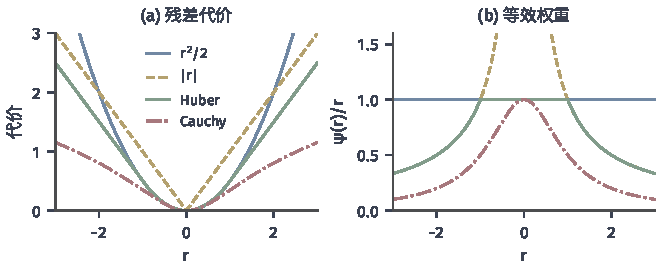
\includegraphics[width=112mm]{figures/03-optimization-evolution-and-signals/01-optimization/matplotlib/c8-residual-losses/figure.pdf}
  \caption{残差代价及其等效权重。(a)~平方$r^2/2$、绝对值$|r|$、Huber损失（$\delta=1$）与Cauchy代价$\tfrac12\log(1+r^2)$。(b)~把每种代价写成$\tfrac12\rho(r^2)$后的权重$\rho'(r^2)=\psi(r)/r$，其中$\psi$是代价对$r$的导数：平方代价对所有残差权重为$1$，绝对值的权重$1/|r|$在零残差处无界，Huber权重为$\min\{1,1/|r|\}$，Cauchy权重$1/(1+r^2)$随残差增大趋于零。}
  \label{fig:opt-fit-residual-losses}
\end{figure}

计价方式直接改变答案。用一个常数$w$拟合三个读数$0,0,10$：平方代价$\sum_i(w-y_i)^2/2$在均值$w=10/3$处最小；绝对值代价$\sum_i|w-y_i|$在中位数$w=0$处最小；对$\delta=1$的Huber损失，若$0\le w\le1$，前两项各为$w^2/2$，第三项为$(10-w)-\tfrac12$，和为$w^2-w+9.5$，在$w=\tfrac12$处导数为零，而目标是凸的，所以$w=\tfrac12$是全局最小点。远离其他读数的$10$把均值拉到$10/3$，对Huber解只施加了大小为$\delta$的有界推力。

每个读数还可以带一个给定的正权重$\omega_i$，表示我们对该读数的信任程度，此时数据代价写成$\sum_i\omega_i\ell(r_i)$。本章把$\omega_i$当作事先确定的量；怎样由噪声的统计模型推出损失与权重，属于统计推断的问题，可参考\BookChapterRef{chap:statistical-inference}{卷四“统计推断”章}。

\paragraph{插值与拟合是不同的任务}
要求$Lf=\bm y$精确成立的任务称为\term{插值}（interpolation），它把读数当作硬约束；允许残差并为之计价的任务称为拟合。前者在读数不相容时无解，后者总可以写出目标值。两者的解一般也不同，第~\ref{sec:opt-fit-min-norm-interpolation}小节会给出插值有解的判据，并说明不能用最小二乘解冒充插值。

\paragraph{一般的拟合目标}
把上面的成分合在一起，拟合问题写作
\begin{equation}
  \min_{f\in C}\ \Phi(Lf-\bm y)+\lambda R(f),
  \label{eq:opt-fit-general-objective}
\end{equation}
其中$\Phi:\mathbb R^n\to\mathbb R$是数据代价，例如$\Phi(\bm r)=\sum_i\omega_i\ell(r_i)$；$R:C\to[0,+\infty]$是\term{正则化}（regularization）项，表达读数之外的偏好；$\lambda\ge0$称为\term{正则化参数}（regularization parameter），调节两者的相对分量；候选集合$C$本身还可以包含硬约束，例如$f\ge0$或固定的边界值。插值则写成$\min_{f\in C}R(f)$，s.t.\ $Lf=\bm y$。数据代价、正则化和硬约束分别承担不同的职责，不能互相替代。

\paragraph{不同的正则化控制不同的东西}
以一次函数$f(x)=w_1+w_2x$为例，三种看似相近的“范数”惩罚的是不同的量。系数的欧氏范数$w_1^2+w_2^2$依赖于基的选取，换成基$\{1,x-\tfrac12\}$就会改变；$L^2$范数$\int_0^1f^2\,\mathrm dx=w_1^2+w_1w_2+w_2^2/3$度量函数本身的大小；导数半范数$\int_0^1(f')^2\,\mathrm dx=w_2^2$只惩罚斜率，对所有常数函数都等于零。最后一种是\term{半范数}（seminorm）：它满足齐次性与三角不等式，却在非零的常数上取零，因此单独使用时不会限制函数的整体高度。第~\ref{sec:opt-fit-linear-basis}小节将看到，在同一组数据上这三种惩罚会选出不同的函数。

\paragraph{有限正则参数不等于精确约束}
有人把约束$Lf=\bm y$换成罚项$\rho\|Lf-\bm y\|_2^2$，期望在$\rho$足够大时得到同样的解。一维例子说明这一般不成立：在约束$w=1$下极小化$w^2$，答案是$w=1$；而$w^2+\rho(w-1)^2$的极小点是$w=\rho/(1+\rho)$，对任何有限的$\rho>0$都严格小于$1$。罚项只能在极限$\rho\to\infty$下逼近约束，有限的正则参数对应的是另一个问题。

\subsection{显式正则化与参数衰减}
\label{sec:opt-fit-weight-decay}

上一小节把偏好写进目标~\eqref{eq:opt-fit-general-objective}。训练神经网络时还有另一种常见做法：目标只含数据项，而在每次更新时把参数乘以略小于$1$的因子。两种做法都叫“正则化”，它们是否等价？本小节在同一个数据目标$F(\bm w)$上逐项比较。

\paragraph{两种更新规则}
Adam维护一阶与二阶历史统计$\bm m,\bm v$，以衰减系数$\beta_1,\beta_2\in[0,1)$更新，并做零初始化的偏差校正，其构造见第~\ref{chap:opt-stochastic-block}章；这里只需要它的一轮更新形式。记第$t$轮（$t=1,2,\dots$）读入的方向为$\bm g^{(t)}$，所有平方、开方与除法逐坐标进行：
\[
  \begin{gathered}
  \bm m^{(t)}=\beta_1\bm m^{(t-1)}+(1-\beta_1)\bm g^{(t)},\qquad
  \bm v^{(t)}=\beta_2\bm v^{(t-1)}+(1-\beta_2)(\bm g^{(t)})^2,\\
  \widehat{\bm m}=\frac{\bm m^{(t)}}{1-\beta_1^t},\qquad
  \widehat{\bm v}=\frac{\bm v^{(t)}}{1-\beta_2^t}.
  \end{gathered}
\]
第一种做法把$\tfrac\lambda2\|\bm w\|_2^2$加进目标，于是$\bm g^{(t)}=\nabla F(\bm w^{(t-1)})+\lambda\bm w^{(t-1)}$，更新为$\bm w^{(t)}=\bm w^{(t-1)}-\eta\,\widehat{\bm m}/(\sqrt{\widehat{\bm v}}+\varepsilon)$。第二种做法是AdamW\scite{loshchilov2019adamw}，称为\term{解耦权重衰减}（decoupled weight decay）：统计只读取数据梯度$\bm g^{(t)}=\nabla F(\bm w^{(t-1)})$，衰减另外施加，
\begin{equation}
  \bm w^{(t)}=(1-\eta\lambda)\bm w^{(t-1)}-\eta\,\frac{\widehat{\bm m}}{\sqrt{\widehat{\bm v}}+\varepsilon}.
  \label{eq:opt-fit-adamw}
\end{equation}
这里约定两项都由更新前的参数与本轮统计算出。若先完成梯度步、再把整个结果乘以$1-\eta\lambda$，梯度项也会被缩放，得到的是另一条更新规则；两者共用“权重衰减”这个名称，却不能混用。

\paragraph{一个可复算的首步}
取标量参数$w^{(0)}=1$，两个历史矩为零，数据梯度恒为零，$\eta=0.1$，$\lambda=2$，$\varepsilon=1$。AdamW的统计只看到零梯度，$\widehat m=0$，由式~\eqref{eq:opt-fit-adamw}，$w^{(1)}=(1-0.2)\cdot1=0.8$。把二次正则加入目标后，$g^{(1)}=\lambda w^{(0)}=2$，偏差校正给出$\widehat m=2$、$\widehat v=4$，于是$w^{(1)}=1-0.1\cdot2/(2+1)=14/15$。同一个$\lambda$，两种做法在第一步就给出不同的结果。

图~\ref{fig:opt-fit-decay-vs-l2}(a)把这一比较延续到$30$步（$\beta_1=0.9$，$\beta_2=0.999$）。AdamW每步乘以$0.8$，几何地趋于零；在加二次正则的Adam中，正则梯度$2w$要先除以二阶统计的平方根；$\beta_2=0.999$使这个统计近似是全部历史梯度平方的平均，停留在早期较大梯度的量级，于是位移并不随$w$成比例缩小，曲线近似直线下行，在第$19$与第$20$步之间越过零。正则项的作用被逐坐标的归一化改写了，这是两种做法的根本差别。

\begin{figure}[!htbp]
  \centering
  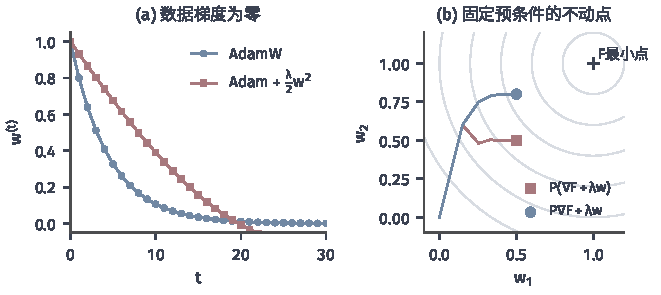
\includegraphics[width=112mm]{figures/03-optimization-evolution-and-signals/01-optimization/matplotlib/c8-decay-vs-l2/figure.pdf}
  \caption{显式二次正则与解耦衰减。(a)~数据梯度恒为零时的标量迭代，$w^{(0)}=1$，$\eta=0.1$，$\lambda=2$，$\varepsilon=1$，$\beta_1=0.9$，$\beta_2=0.999$：AdamW（圆点）每步乘$0.8$；加入$\tfrac\lambda2w^2$后的Adam（方块）首步为$14/15$，此后近似线性下降并越过零。(b)~固定预条件$\bm P=\operatorname{diag}(1,4)$下，对$F(\bm w)=\tfrac12\|\bm w-(1,1)\|_2^2$、$\lambda=1$、$\eta=0.15$从原点出发的两条轨迹：更新$\bm w-\eta\bm P(\nabla F+\lambda\bm w)$收敛到$(\tfrac12,\tfrac12)$，更新$\bm w-\eta(\bm P\nabla F+\lambda\bm w)$收敛到$(\tfrac12,\tfrac45)$。灰色圆是$F$的等值线。}
  \label{fig:opt-fit-decay-vs-l2}
\end{figure}

\paragraph{需要逐项记录的设置}
实际使用时，是否对偏置、归一化层参数施加衰减，各实现并不一致，所以要明确列出受衰减的参数。还要注意收缩系数的写法：有的实现写成$1-\eta^{(t)}\lambda$，衰减随学习率调度一起变化；有的写成与步长无关的$1-\lambda'$。在变步长下，$T$步累计的收缩因子分别是$\prod_{t}(1-\eta^{(t)}\lambda)$与$(1-\lambda')^T$，即使首步相同，后面也会分开。

\paragraph{固定预条件下的直接计算}
历史统计使上面的比较难以写成闭式。把Adam的逐坐标缩放换成固定的正定对角矩阵$\bm P$，差别就能精确算出。比较两种更新：
\[
  \text{(i)}\ \ \bm w^+=\bm w-\eta\bm P\bigl(\nabla F(\bm w)+\lambda\bm w\bigr),\qquad
  \text{(ii)}\ \ \bm w^+=\bm w-\eta\bigl(\bm P\nabla F(\bm w)+\lambda\bm w\bigr).
\]
(i)是对$F+\tfrac\lambda2\|\bm w\|_2^2$的预条件梯度步，不动点满足$\nabla F+\lambda\bm w=\bm 0$。(ii)可以改写为$\bm w-\eta\bm P\bigl(\nabla F+\lambda\bm P^{-1}\bm w\bigr)$，它是对另一个目标$F+\tfrac\lambda2\bm w^\top\bm P^{-1}\bm w$的预条件梯度步，不动点满足$\nabla F+\lambda\bm P^{-1}\bm w=\bm 0$。所以在固定预条件下，解耦衰减等价于把欧氏惩罚换成按$\bm P^{-1}$加权的惩罚：缩放大的坐标，受到的有效惩罚反而小。

取$F(\bm w)=\tfrac12\|\bm w-(1,1)^\top\|_2^2$、$\lambda=1$、$\bm P=\operatorname{diag}(1,4)$验算。(i)的不动点解$2\bm w=(1,1)^\top$，即$(\tfrac12,\tfrac12)$；(ii)的不动点逐坐标解$1\cdot(w_1-1)+w_1=0$与$4(w_2-1)+w_2=0$，得$(\tfrac12,\tfrac45)$。图~\ref{fig:opt-fit-decay-vs-l2}(b)中两条轨迹分别停在这两点。$\bm P$随历史变化时，(ii)连这样一个固定的等价目标也没有，需要单独分析。因此报告结果时应同时写明数据目标、显式正则目标和实际的更新规则，并按事先规定的评价目标比较，不能仅凭“都用了$\lambda$”认为它们求解的是同一个问题。
